\documentclass[../main.tex]{subfiles}
\begin{document}

Die Vektor Embeddings werden selten isoliert betrachtet, sondern als Teil eines Vektorraums.
In diesem Raum wird durch die Embeddings Richtung und Entfernung Bedeutung zugewiesen.
So liegt Text, der ähnliche Semantik hat, nahe aneinander in seiner Embedding Darstellung in solch einem Vektorraum.
Außerdem stellt das Verhältnis zwischen zwei Vektoren semantische Konzepte dar und es können Achsen gebildet werden, auf die die Embeddings projeziert werden und damit verallgemeinernd Konzepte erfassen, wie in Abbildung \ref{fig:embeddingspace} zu erkennen.
\cite{heimerl2018interactive,mikolov2013efficient}

\begin{figure}[ht]
    \centering
    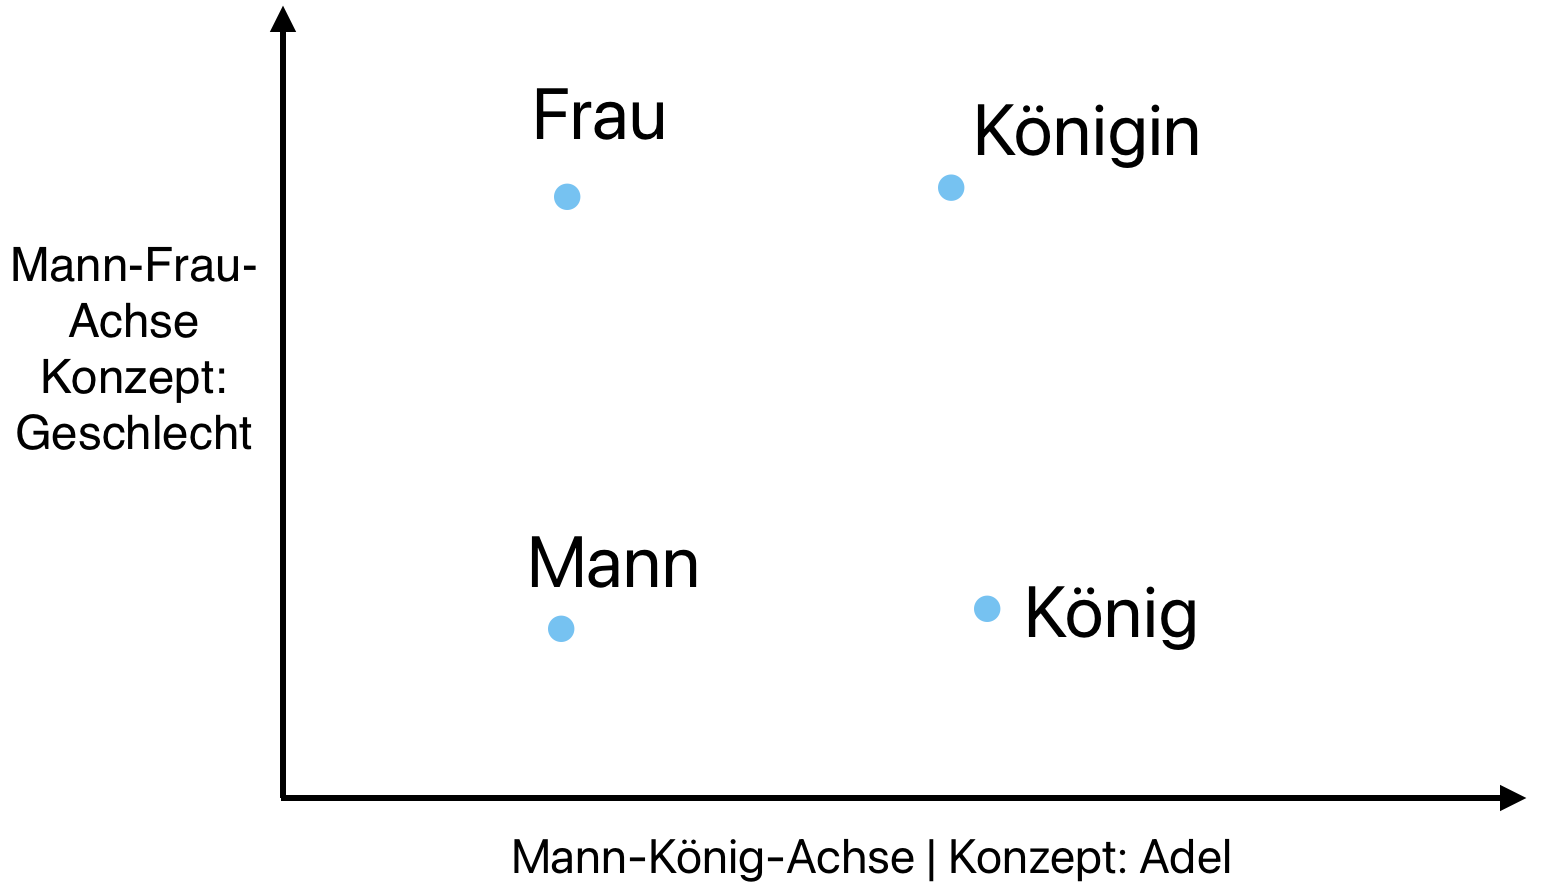
\includegraphics[scale=.23]{"bilder/embeddingspace.png"}
    \caption{Darstellung von einem ausgedachten Vektor Embedding Raum über zwei Konzeptachsen (eigene Darstellung)}
    \label{fig:embeddingspace}
\end{figure}

Um einen Vektor Embedding Raum sinnvoll aufzubauen, ist eine einheitliche Methode zur Generierung von Embeddings nötig, in der die Bedeutungszuweisung von Richtungen kohärent zwischen den Embeddings ist.
Dafür können \glspl{LLM} durch ihr Textverständnis genutzt werden, um aus einer Texteingabe ein Ausgabe-Vektor Embedding zu erzeugen.
\cite{zhang2023language}

\end{document}